%!TEX root = main.tex
\newpage
\chapter{StackLetter -- personalizovaný informačný bulletin pre Stack Exchange}

\textit{StackLetter} je systém pre vytváranie a rozosielanie personalizovaných informačných bulletinov vrámci platformy
Stack Exchange. Tento systém vznikol ako súčasť spolupráce autora tejto práce a Bc. Matúša Saláta~\cite{Salat2018} vrámci
dvoch diplomových prác riešených v akademickom roku 2016/17 a 2017/18. Celý systém sa skladá
z viacerých spolupracujúcich modulov, ktoré však boli vyvíjané samostatne a sú od seba navzájom nezávislé. Rozdelenie
systému na nezávislé moduly umožňuje rýchlejší vývoj, ako aj možnosť jednoduchého rozširovania systému v budúcnosti.
Architektonický prehľad celého systému znázorňuje obrázok~\ref{fig:architecutre-overview}. Ďalej v tejto práci opisujem
len mnou navrhnuté moduly.

\begin{figure}[H]\begin{center}
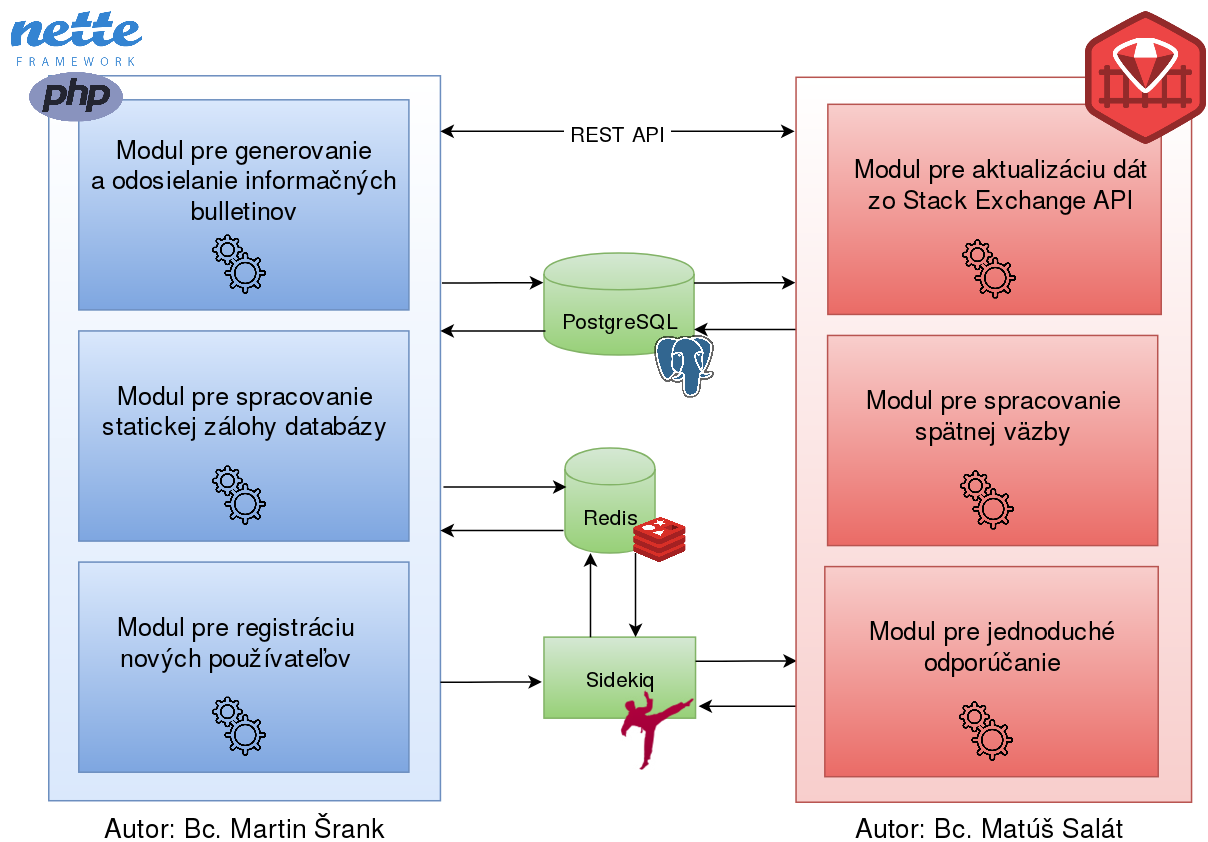
\includegraphics[scale=0.32]{architecture-overview}
\caption{Architektonický prehľad systému StackLetter. \label{fig:architecutre-overview}}\end{center}
\end{figure}

\section{Prehľad modulov}

\textbf{Modul pre registráciu nových používateľov}\\
Tento modul predstavuje používateľmi viditeľnú časť systému. Prostredníctvom webovej stránky systému
-- \url{www.stackletter.com} -- sa používatelia môžu prihlásiť k odoberaniu informačného bulletinu pre niektoré
z ponúkaných komunít platformy Stack Exchange, ako aj spravovať svoje nastavenia týkajúce sa odosielania informačných
bulletinov.\\
Používatelia sa prihlasujú prostredníctvom svojho Stack Exchange konta využitím protokolu OAuth.

\begin{figure}[H]\begin{center}
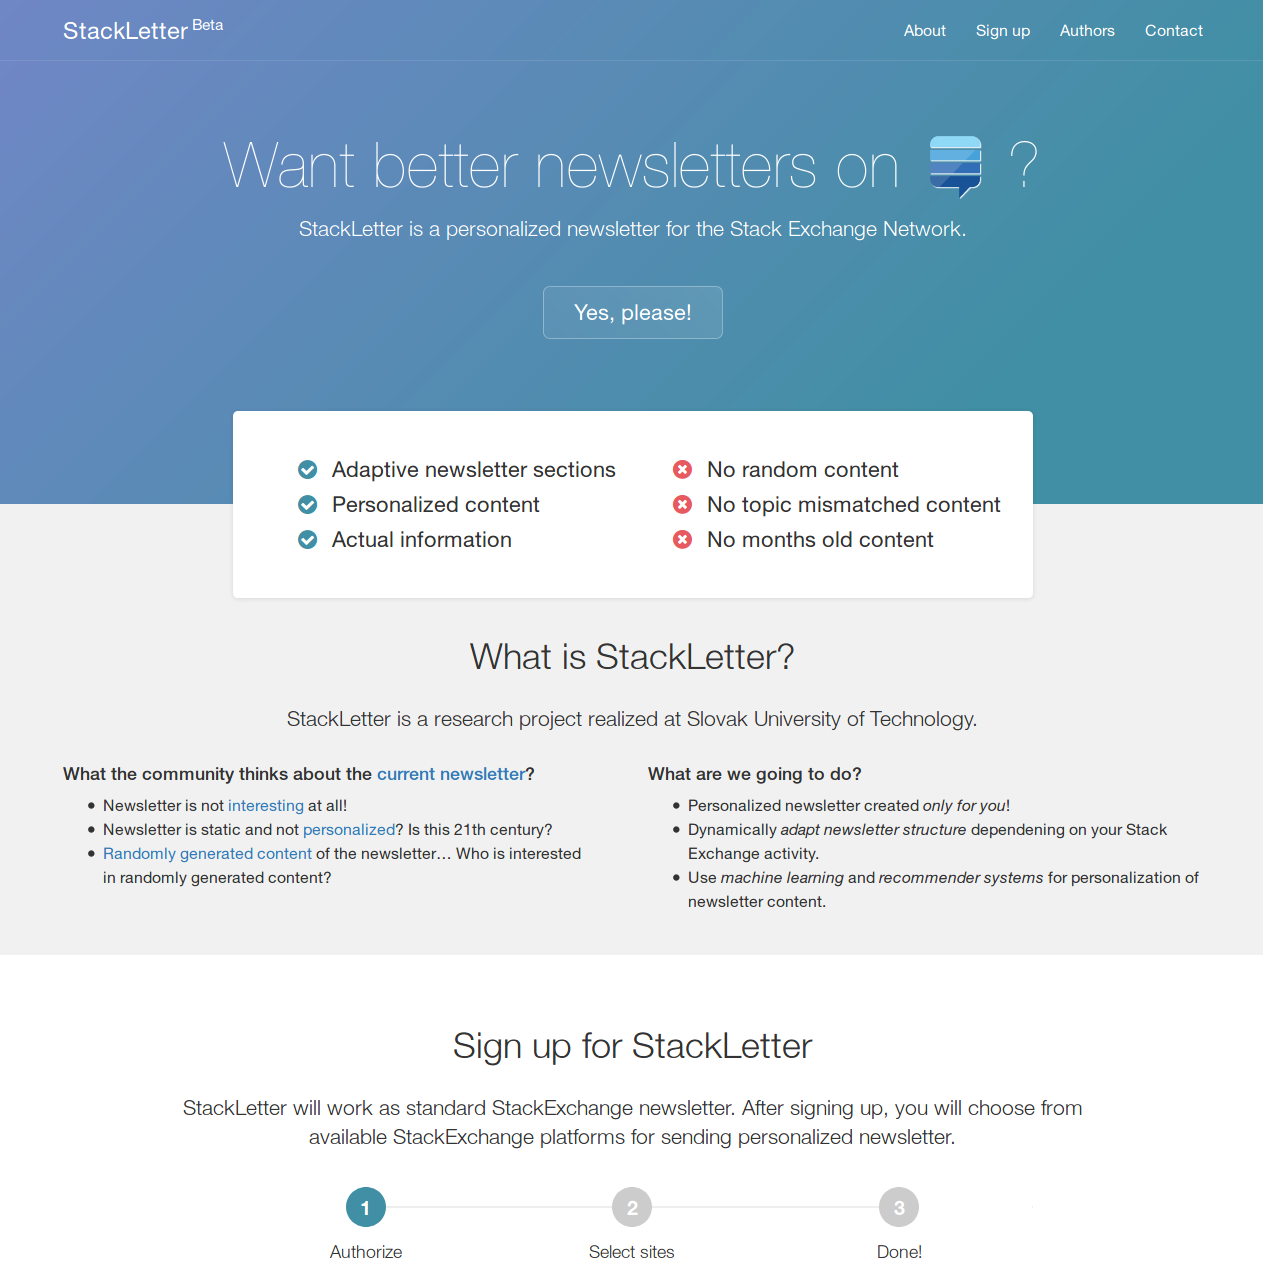
\includegraphics[scale=0.35]{stackletter-screenshot}
\caption{Snímka registračnej stránky StackLetter.com. \label{fig:stackletter.com}}\end{center}
\end{figure}

\textbf{Modul pre generovanie a odosielanie informačných bulletinov}\\
Tento modul je zodpovedný za samotné zostavovanie a odosielanie informačných bulletinov jednotlivým zaregistrovaným
používateľom. Prostredníctvom REST API komunikuje s modulmi pre zostavovanie odporúčaní a štruktúry informačných bulletinov
a na základe ich odpovedí vygeneruje naformátované informačné bulletiny, ktoré sú následne rozosielané prostredníctvom služby
SendGrid\footnote{\url{https://sendgrid.com}}.

\textbf{Modul pre spracovanie statickej zálohy databázy}\\
Modul bol navrhnutý a implementovaný za účelom rýchleho a efektívneho importovania počiatočných dát platformy Stack Exchange
dostupných vo forme XML exportu do našej internej reprezentácie v databáze PostgreSQL.

\textbf{Modul pre personalizované odporúčanie}\\
Modul zabezpečuje samotné vytváranie personalizovaných zoznamov odporúčaní prostredníctvom metódy navrhnutej v tejto práci.
Podrobne sa realizácii tohto modulu venujeme v kapitole~\ref{impl:rec}.

Podrobný technický a architektonický popis jednotlivých modulov sa nachádza
v prílohe~\ref{tech-doc} -- \textit{Technická dokumentácia systému StackLetter}.

\section{Použité technológie a služby}

\begin{my_itemize}
\item{Jednotlivé moduly zabezpečujúce infraštruktúru systému StackLetter sú implementované v~jazyku PHP\footnote{\url{https://php.net}}
verzie~7.1 s použitím MVC frameworku Nette~2.4\footnote{\url{https://nette.org}}.}
\item{Systém na ukladanie dát využíva relačný databázový systém PostgreSQL vo verzii 9.6 a~vnútropamäťové dátové úložisko Redis
vo verzii 4.0.}
\item{Systém komunikuje s platformou Stack Exchange prostredníctvom Stack Exchange API v2.2 a~vykonáva autentifikáciu
používateľov prostredníctvom protokolu OAuth 2.0.}
\item{Na hromadné odosielanie informačných bulletinov používateľom prostredníctovm e-mailu je využitá služba SendGrid.}
\item{Modul pre zostavovanie personalizovaných informačných bulletinov so zameraním na diverzitu je implementovaný
v jazyku Python 3.6 s použitím knižníc scikit-learn, numpy (pre prácu s modelmi) a Flask (pre implementáciu REST API).}
\end{my_itemize}


\section{Realizácia personalizovaného odporúčania}
\label{impl:rec}

Modul pre personalizované odporúčanie je navrhnutý ako samostatný modul, ktorý poskytuje REST API pre komunikáciu
s modulom pre generovanie a odosielanie informačných bulletinov. Vďaka tomu je možné do budúcnosti jednoducho nahradiť
tento modul iným modulom bez potreby výrazných zásahov do existujúcich častí systému.

\subsection{Zostavenie LDA a TF-IDF modelov}

\textbf{Slovník}\\
Pre LDA a TF-IDF modely využívané v navrhnutej metóde sme vytvorili slovnú zásobu pozostávajúcu z 500 tisíc náhodne vybraných
otázok z komunity Stack Overflow. Texty prešli predspracovaním v podobe odstránenia formátovania (HTML tagov), diakritiky,
anglických stop slov. Minimálna dokumentová frekvencia bola stanovená na $5$ a maximálna dokumentová frekvencia na $99\%$.
Okrem toho bola maximálna veľkosť slovníka stanovená na 150 tisíc výrazov, pričom skutočný počet výrazov bol cca 152 tisíc.
Na vytvorenie slovníku bol použitý \textit{CountVectorizer} z~knižnice \textit{scikit-learn}.

\textbf{Nastavenie a trénovanie LDA modelu}\\
Pravdepodobne najdôležitejším parametrom pri Latentnej Dirichletovej Alokácii je určenie počtu LDA tém. Pre určenie počtu sme
na testovacie dáta (náhodne vybraných stotisíc otázok) opakovane aplikovali klastrovanie prostredníctvom metódy K-Means, pričom
hodnotu $k$ sme vyberali z intervalu $<20,100>$. Pre každú hodnotu $k$ sme následne vypočítali priemerný siluetový koeficient
(viď.~Obr.~\ref{fig:silhouette}). Na základe tejto analýzy sme stanovili počet LDA tém na 50.

\begin{figure}[H]\begin{center}
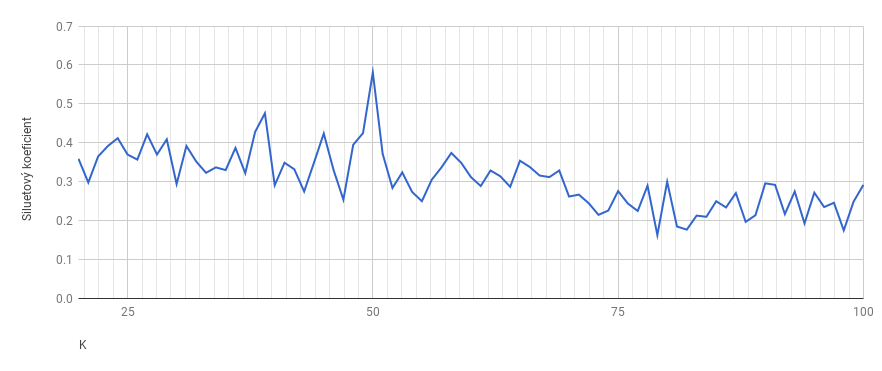
\includegraphics[scale=0.53]{silhouette}
\caption{Siluetový koeficient vzhľadom na $K$. \label{fig:silhouette}}\end{center}
\end{figure}

LDA model sme natrénovali na vzorke stotisíc náhodne zvolených otázok zo Stack Overflow, pričom sme využili slovník výrazov
vytvorený v predošlom kroku. Ostatné parametre modelu boli nastavené tak, ako boli definované v kapitole~\ref{design:lda-setup}.
Bola použitá implementácia LDA z~knižnice \textit{scikit-learn}.

\textbf{TF-IDF model}\\
TF-IDF model zostavujeme zvlášť pre každého používateľa z otázok, s ktorými interagoval, a to pri každom pretrénovaní používateľských
modelov, ktoré sa vykonáva raz denne pre používateľov s denným informačným bulletinom a raz týždenne pre používateľov s týždenným
bulletinom. Využíva sa implementácia \textit{TfidfTransformer} z~knižnice \textit{scikit-learn}.


\subsection{Vytváranie modelov otázok a používateľov}

\textbf{Model otázky}\\
Model otázky sa skladá z troch vektorov: 1) vektor značiek (tagov), ktorými je otázka označená, 2) vektor reprezentujúci
distribúciu otázky vrámci LDA tém a 3) TF vektor. Vektor značiek sa vytvára za behu priamo požiadavkou do databázy. TF vektor
sa tiež vytvára až za behu z textu otázky, nakoľko sa jedná o veľmi rýchlu operáciu. Vektor distribúcie LDA tém sa vytvára
vždy pri vzniku novej otázky, alebo po interakcii používateľa s otázkou, pre ktorú ešte nebol vytvorený. Tento vektor
sa po vytvorení ukladá do databázy. Vytváranie modelov pre novo vzniknuté otázky sa vykonáva raz denne.

\textbf{Model používateľa}\\
Model používateľa sa nevytvára za behu, ale sa perzistuje v binarizovanej podobe do súboru, odkiaľ sa v prípade použitia
načítava. Model používateľa sa delí na model záujmu a model expertízy, pričom tie sa vytvárajú z modelov otázok, s ktorými
používateľ interagoval.

Každý model sa skladá z vektoru značiek, ktorý predstavuje relatívne zastúpenie značiek v otázkach, s ktorými používateľ interagoval,
normalizovaných do intervalu $<0,1>$; vektoru LDA tém, ktorý je vytvorený analogicky a tiež normalizovaný do intervalu $<0,1>$,
a matice TF vektorov z modelov príslušných otázok. Z tejto matice sa následne predpočíta aj matica TF-IDF.

\textbf{Aktualizácia modelov používateľov}\\
Model používateľa sa aktualizuje v pravidelných intervaloch na základe jeho preferencie prijímania informačných bulletinov, teda
denne alebo týždenne. Pre zachytenie meniacich sa záujmov používateľa v čase (viď kapitola~\ref{design:freshness}) sa využíva
faktor úpadku, ktorý sa počíta na základe relatívneho počtu aktivity za obdobie od poslednej aktualizácie modelu voči
celkovému množstvu používateľovej aktivity.

Pri aktualizácii modelu používateľa sa najprv týmto faktorom úpadku prenásobia vektory reprezentujúce doterajšiu aktivitu
a následne sa k nim prirátajú hodnoty z obdobia od poslednej aktualizácie. Vektory značiek a LDA tém sa následne nanovo
normalizujú a z TF matice sa nanovo predpočíta matica TF-IDF.

\textbf{Použitie modelov používateľov v sekciách informačného bulletinu}\\
Na základe sekcie informačného bulletinu, pre ktorú sa vytvára zoznam odporúčaní sa využíva buď záujmový alebo
expertízny model používateľa, alebo oba, ako popisuje tabuľka~\ref{tab:sections}.

\begin{table}[h]
\label{tab:sections}
\centering
\caption{Sekcie informačného bulletinu a k nim prislúchajúce modely používateľa}
\begin{tabular}{|m{7cm}|>{\centering\arraybackslash}m{2.5cm}|>{\centering\arraybackslash}m{2.6cm}|}
\hline
\textbf{Sekcia} & \textbf{Záujmový model} & \textbf{Expertízny model} \\\hline
Najnovšie otázky               & ×  & -- \\\hline
Užitočné otázky                & ×  & -- \\\hline
Otázky čakajúce na odpoveď     & -- & ×  \\\hline
Populárne nezodpovedané otázky & -- & ×  \\\hline
Vysoko diskutované otázky      & ×  & ×  \\\hline
Vysoko diskutované odpovede    & ×  & ×  \\\hline
Zaujímavé odpovede             & ×  & ×  \\\hline
\end{tabular}
\end{table}

\textbf{Komunitný model používateľov}\\
V prípade, že používateľský model neobsahuje dostatočné množstvo aktivity pre zostavenie relevantných odporúčaní,
sa použije tzv. \textit{Komunitný model používateľov}. Ten je presne analogický so štandardným modelom používateľa,
no skladá sa nie z aktivity konkrétneho používateľa, ale zo všetkých položených otázok a odpovedí v celom CQA systéme.
Rovnako ako štandardné používateľské modely sa aj komunitný model aktualizuje denne aj s aplikáciou faktoru úpadku.
